
% This must be in the first 5 lines to tell arXiv to use pdfLaTeX, which is strongly recommended.
\pdfoutput=1
% In particular, the hyperref package requires pdfLaTeX in order to break URLs across lines.

\documentclass[11pt]{article}

% Change "review" to "final" to generate the final (sometimes called camera-ready) version.
% Change to "preprint" to generate a non-anonymous version with page numbers.
\usepackage[review]{acl}

% Standard package includes
\usepackage{times}
\usepackage{latexsym}

% For proper rendering and hyphenation of words containing Latin characters (including in bib files)
\usepackage[T1]{fontenc}
% For Vietnamese characters
% \usepackage[T5]{fontenc}
% See https://www.latex-project.org/help/documentation/encguide.pdf for other character sets

% This assumes your files are encoded as UTF8
\usepackage[utf8]{inputenc}

% This is not strictly necessary, and may be commented out,
% but it will improve the layout of the manuscript,
% and will typically save some space.
\usepackage{microtype}

% This is also not strictly necessary, and may be commented out.
% However, it will improve the aesthetics of text in
% the typewriter font.
\usepackage{inconsolata}

%Including images in your LaTeX document requires adding
%additional package(s)
\usepackage{graphicx}
\usepackage{setspace}
\usepackage{graphicx}
\usepackage{listings}
\usepackage{xcolor}
\usepackage{subcaption}
\usepackage{import}

% Add this line to define \textrussian command
\newcommand{\textrussian}[1]{\foreignlanguage{russian}{#1}}

\lstset{
    language=Python,
    breaklines=true,
    basicstyle=\ttfamily,
    keywordstyle=\color{blue},
    linewidth=0.5\textwidth,  % Set the width to 90% of the text width
}
\usepackage{graphicx}
\graphicspath{{../plots/}}


\begin{document}

\nolinenumbers  % Add this line to ensure line numbers are turned off


\title{NLP Course Report}
\author{Hans Peter Lyngsøe, pvr448}

\maketitle

\section{Week 1}
% (a) Explore the dataset from https://huggingface.co/datasets/coastalcph/tydi_xor_rc. 
% Familiarize yourself with the dataset card, download the dataset and explore its columns. 
% Summarize basic data statistics for training and validation data in each of the languages 
% Finnish (fi), Japanese (ja) and Russian (ru).
\begin{enumerate}
    \item[(a)] 

    Basic statistics:
    \begin{itemize}
        \item the data is quite evenly distributed across the 3 languages.
        \item We note that there are more answerable than unanswerable by a factor of 10-1.Which means we accuracy becomes a meaningless measure for performance.
        \item train\_set: 15326
        \item val\_set: 3028
    \end{itemize}

    \begin{figure}[ht]
        \centering
        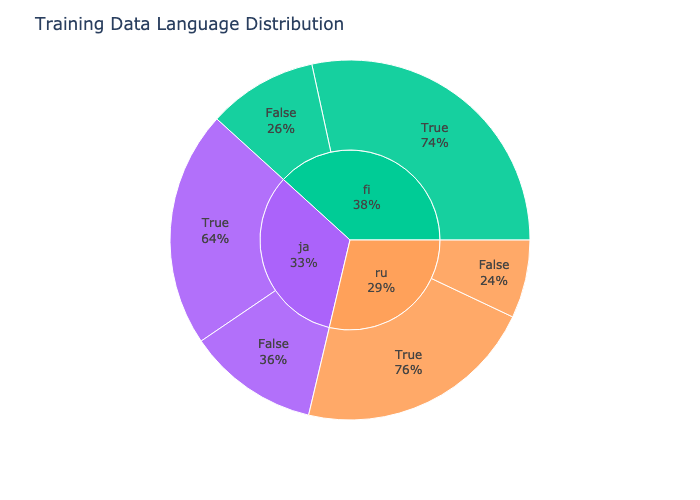
\includegraphics[width=0.3\textwidth]{week1_a_dataset.png}
        \caption{Distribution of labels in the dataset}
        \label{fig:label_distribution}
    \end{figure}

    \begin{figure}[ht]
        \centering
        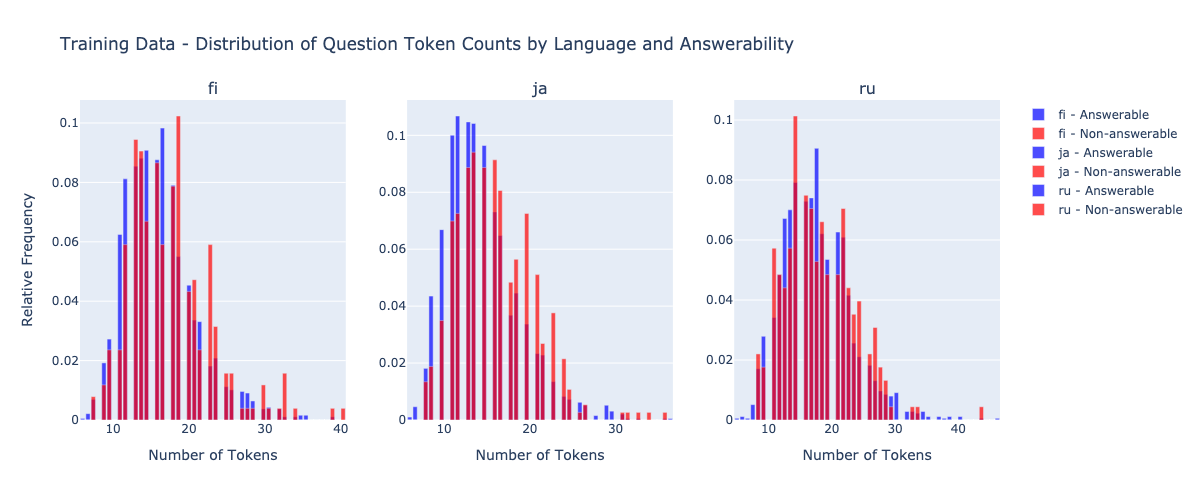
\includegraphics[width=0.5\textwidth]{week1_a_lang_token_distribution_normalized.png}
        \caption{normalized Histogram for token count(using llama3 tokenizer) of answerable/unanswerable questions in the dataset}
        \label{fig:language_distribution}
    \end{figure}

    % (b) For each of the languages Finnish, Japanese and Russian, report the 5 most common 
    % words in the questions from the training set. What kind of words are they?
    \item[(b)] 

    In order to get a faithful representation of the most meaningful words, we opt to filter out stopwords arguing that these words are not meaningful and does not carry information about the question.
    We use the NLP library spacy that provides and index of stopwords for each language. Additionally we remove common symbols like '.' and '?'.

    we use the fact that both finnish and russian uses spaces to seperate their words, and thus we can extract distinct words using the space as delimiter.
    Japanese is somewhat different as a language, and it is unclear whether naive splitting on space is meaningful. Thus we use a japanese speific tokenizer to parse sentences into words.
    we get the following results:

    \begin{figure}[t]
        \centering
        \begin{subfigure}[b]{0.1\textwidth}
            \centering
            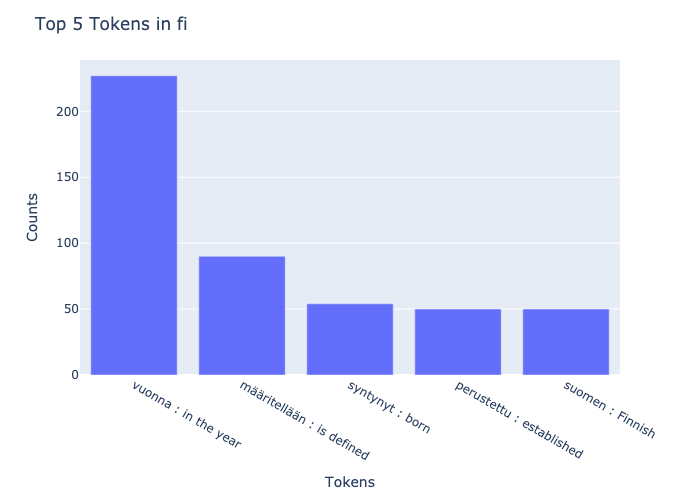
\includegraphics[width=\textwidth]{week1_b_top_5_tokens_fi.png}
            \caption{Finnish}
            \label{fig:top_5_tokens_fi}
        \end{subfigure}
        \hfill
        \begin{subfigure}[b]{0.1\textwidth}
            \centering
            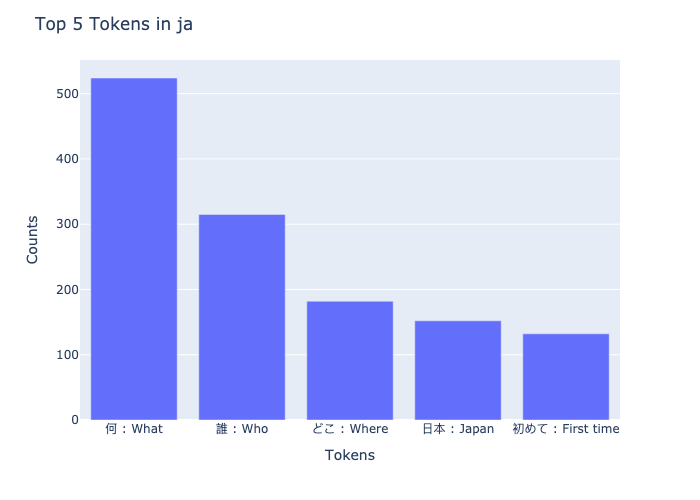
\includegraphics[width=\textwidth]{week1_b_top_5_tokens_ja.png}
            \caption{Japanese}
            \label{fig:top_5_tokens_ja}
        \end{subfigure}
        \hfill
        \begin{subfigure}[b]{0.1\textwidth}
            \centering
            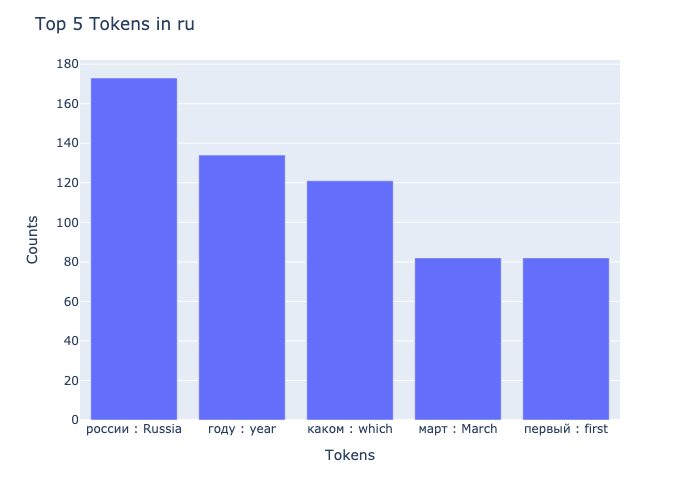
\includegraphics[width=\textwidth]{week1_b_top_5_tokens_ru.png}
            \caption{Russian}
            \label{fig:top_5_tokens_ru}
        \end{subfigure}
        \caption{Top 5 tokens in Finnish, Japanese, and Russian}
        \label{fig:top_5_tokens_all}
    \end{figure}

    NOTE: todo use an embedding model to get a sense for the meaning of the words, consider how you do tokenization and 
    what the implications are. what are words and what are stopwords

    % (c) Implement a rule-based classifier that predicts whether a question is answerable 
    % or impossible, only using the document (context) and question. You may use machine 
    % translation as a component. Use the answerable field to evaluate it on the validation set. 
    % What is the performance of your classifier for each of the languages Finnish, Japanese and Russian?
    \item[(c)] 
    
    As a simple rule based approach explore the relationship between word/token count and answerability in the training set. 
    We expect that as a rough heuristic that longer questions are harder to answer. 
    In the appendix, we provide scatter plots for each language. See Figures~\ref{fig:scatter_week1_c_fi}, \ref{fig:scatter_week1_c_ja}, and \ref{fig:scatter_week1_c_ru} show the scatter plots for Finnish, Japanese, and Russian data respectively.
    based on this information, we decide to make a rule based classifier that predicts unanwerable for questions above a specific length that is different for each language.
    We select this length by looking at the training distribution. 
    ('ja': 10, 'ru': 15, 'fi': 9)

    we get the following results on the validation set:

    %% ja: {'accuracy': 0.5877192982456141, 'balanced_accuracy': 0.53745129167268, 'f1': 0.6907894736842105, 'precision': 0.6542056074766355, 'recall': 0.7317073170731707}
    %% ru: {'accuracy': 0.7121212121212122, 'balanced_accuracy': 0.4964788732394366, 'f1': 0.831858407079646, 'precision': 0.7157360406091371, 'recall': 0.9929577464788732}
    %% fi: {'accuracy': 0.6912878787878788, 'balanced_accuracy': 0.5132645803698435, 'f1': 0.81068524970964, 'precision': 0.7255717255717256, 'recall': 0.9184210526315789}
    %% all: {'accuracy': 0.6630434782608695, 'balanced_accuracy': 0.5284132271513975, 'f1': 0.783418723800652, 'precision': 0.7031772575250836, 'recall': 0.8843322818086226}
    \begin{table}[ht]
        \centering
        \begin{tabular}{|l|c|c|c|c|}
            \hline
            Language & Balanced Accuracy & F1 Score & Precision & Recall \\
            \hline
            All & 0.5284 & 0.7834 & 0.7032 & 0.8843 \\
            Finnish (fi) & 0.5133 & 0.8107 & 0.7256 & 0.9184 \\
            Japanese (ja) & 0.5375 & 0.6908 & 0.6542 & 0.7317 \\
            Russian (ru) & 0.4965 & 0.8319 & 0.7157 & 0.9930 \\
            \hline
        \end{tabular}
        \caption{Performance metrics of the rule-based classifier on the validation set}
        \label{tab:classifier_performance}
    \end{table}

    There are many downsides to this approach: 
    first of all although length might be correlated with answerability this is a vary noisy signal as length is a bad measure of complexity.
    furthermore we are putting a lot of faith in the tokenization step. And the predictions of our model could be meaningfully change with a different tokenization scheme.
    We also note that this is barely better than sampling from a bernoulli distribution with the mean of the answerability in the training data.

\end{enumerate}

\section{Week 37 (9--15 September)}
% Let k be the number of members in your group (k ∈ {1, 2, 3}). Implement k different 
% language models for the questions in the three languages Finnish, Japanese and Russian, 
% as well as for the document contexts in English (total k × 4 language models), using the 
% training data. Evaluate each of them on the validation data, report their performance 
% and discuss the results.

We train 3 different N-Gram models, one for each language.

Curiously enough we find that as we scale the number of tokens in the training data, the performance of the model gets worse.

\begin{table}[ht]
    \centering
    \begin{tabular}{|l|r|r|}
        \hline
        Language & Training Tokens/Words & Perplexity \\
        \hline
        Japanese (ja) & 24,533 & 548.79 \\
        Russian (ru) & 16,526 & 140.53 \\
        Finnish (fi) & 13,013 & 91.90 \\
        Context (English) & 751,154 & 616.85 \\
        \hline
    \end{tabular}
    \caption{Language Model Performance}
    \label{tab:language_model_performance}
\end{table}



\section{Week 38 (16--22 September)}
% Let k be the number of members in your group. For each of the three languages Finnish, 
% Japanese and Russian separately, using the training data, train k different classifiers 
% that receive the document (context) and question as input and predict whether the question 
% is answerable or impossible given the context. Evaluate the classifiers on the respective 
% validation sets, report and analyse the performance for each language and compare the 
% scores across languages.

We train a simple linear layer mapping from an embedding space to the 1d classification space. We use openai's 'text-embedding-ada-002' model to embed the question and context and train on the cocatenation of the two 
This gives us a feature space of dimension 2*1536 = 3072. We train using the binary crossentropy-loss.

\begin{table}[ht]
    \centering
    \resizebox{\textwidth}{!}{%
    \begin{tabular}{|l|l|c|c|c|c|c|c|}
    \hline
    Training & Evaluation & Context & D\_in & Expansion\_factor & Balanced & Precision & Recall \\
    & & & & & Accuracy & & \\
    \hline
    Finnish & Finnish & No & 1536 & 2 & 0.9031 & 0.9825 & 0.9492 \\
    Finnish & Finnish & Yes & 3072 & 2 & 0.7562 & 0.9466 & 0.9767 \\
    Finnish & Japanese & No & 1536 & 2 & 0.8293 & 0.9460 & 0.8904 \\
    Finnish & Japanese & Yes & 3072 & 2 & 0.6366 & 0.8652 & 0.9439 \\
    Finnish & Russian & No & 1536 & 2 & 0.9184 & 0.9943 & 0.9278 \\
    Finnish & Russian & Yes & 3072 & 2 & 0.8556 & 0.9840 & 0.9840 \\
    Finnish & All & Yes & 3072 & 2 & 0.5670 & 0.8981 & 0.9902 \\
    Finnish & All & No & 1536 & 2 & 0.8810 & 0.9775 & 0.9246 \\
    Japanese & Finnish & No & 1536 & 2 & 0.8543 & 0.9716 & 0.9407 \\
    Japanese & Finnish & Yes & 3072 & 2 & 0.5247 & 0.8987 & 0.9958 \\
    Japanese & Japanese & No & 1536 & 2 & 0.7625 & 0.9105 & 0.9519 \\
    Japanese & Japanese & Yes & 3072 & 2 & 0.5244 & 0.8274 & 1.0000 \\
    Japanese & Russian & No & 1536 & 2 & 0.9251 & 0.9919 & 0.9866 \\
    Japanese & Russian & Yes & 3072 & 2 & 0.5896 & 0.9540 & 0.9973 \\
    Japanese & All & Yes & 3072 & 2 & 0.5300 & 0.8903 & 0.9975 \\
    Japanese & All & No & 1536 & 2 & 0.8162 & 0.9574 & 0.9574 \\
    Russian & Finnish & No & 1536 & 2 & 0.6438 & 0.9231 & 0.9661 \\
    Russian & Finnish & Yes & 3072 & 2 & 0.6789 & 0.9313 & 0.9470 \\
    Russian & Japanese & No & 1536 & 2 & 0.7694 & 0.9143 & 0.9412 \\
    Russian & Japanese & Yes & 3072 & 2 & 0.7585 & 0.9098 & 0.9439 \\
    Russian & Russian & No & 1536 & 2 & 0.7045 & 0.9664 & 1.0000 \\
    Russian & Russian & Yes & 3072 & 2 & 0.7955 & 0.9765 & 1.0000 \\
    Russian & All & No & 1536 & 2 & 0.7126 & 0.9314 & 0.9689 \\
    Russian & All & Yes & 3072 & 2 & 0.7436 & 0.9392 & 0.9623 \\
    \hline
    \end{tabular}%
    }
    \caption{Model performance for language-specific training and cross-language evaluation, with and without context}
    \label{tab:model_performance_cross_language}
\end{table}

from the results we see that the russian classifier achieves the highest balanced accuracy followed by the japanese and finnish.
this is unexpected as one would assume the quality of the embeddings would be higher for more common languages spoken online(ja > ru > fi).
but the trend appears to be reversed. Interestingly enough this trend is reversed if we exclusively train on the question embedding. 
Where we observe a meaningfull boost in performance for the finnish and japanese classifiers although we striclty have less information.

additionally to better understand the difficulty of different languages we evaluate the classifier on the validation set of each language, including languages the model was not previously trained on.
Suprinsingly for the finnish and japanese classifiers perform better on the russian validation set than the validation set they were trained on.
to get a better understanding of the impact. The fact that the unilingual classifiers perform so well even on multilingual datasets 

\begin{table}[ht]
    \centering
    \resizebox{\textwidth}{!}{%
    \begin{tabular}{|l|l|c|c|c|c|c|c|}
    \hline
    Training & Evaluation & Context & D\_in & Expansion & Balanced & Precision & Recall \\
    & & & & Factor & Accuracy & & \\
    \hline
    All & Finnish & No & 1536 & 2 & 0.9414 & 0.9933 & 0.9364 \\
    All & Finnish & Yes & 3072 & 2 & 0.9225 & 0.9888 & 0.9343 \\
    All & Japanese & No & 1536 & 2 & 0.6688 & 0.8741 & 0.9840 \\
    All & Japanese & Yes & 3072 & 2 & 0.8663 & 0.9559 & 0.9278 \\
    All & Russian & No & 1536 & 2 & 0.7955 & 0.9765 & 1.0000 \\
    All & Russian & Yes & 3072 & 2 & 0.8810 & 0.9867 & 0.9893 \\
    \hline
    \end{tabular}%
    }
    \caption{Model performance for language-specific and combined training, with and without context}
    \label{tab:model_performance}
\end{table}


\section{Week 39 (23--29 September)}
% We now move from binary classification to span-based QA, i.e. identifying the
% span in the document that answers the question.
% Let k be the number of members in your group. Using the training data in
% Finnish, Japanese and Russian separately, train k different sequence labellers,
% which predict the tokens in a document context that constitute the answer to
% the corresponding question.9 You can decide whether to train one model per
% language or a single model for all three languages. Evaluate using a sequence la-
% belling metric on the validation set, report and analyse the performance for each
% language and compare the scores across languages. Note that if the question is
% unanswerable, a correct output must be empty (contain no tokens).

We experiment with various sequence labeling models encoder-decoder models. 
We finetune, distilbert, and deberta\_V3 and in both cases we get a perfect match of 50%

However we note that there is a meaningful discrepancy between how the model performs on finnish vs russian and japanese. As distilbert and deberta is not explicitly intended for multilingual tasks.
Thus we opt for using the mt5 base model that is a t5 encoder decoder model that is trained on both japanese, russian and finnish along with many other languages.
Instead of doing a whole finetune we freeze the weights and use a lora adapter 


\begin{itemize}
    \item 
    finetune for one language only and compare with the performance when training on all languages
    measure before and after finetuning perf on validation set.
\end{itemize}

we use the same metrics as established in the squad v1 paper. \cite{rajpurkar-etal-2018-know}.

We experiment with finetuning different models including distilbert, deberta\_v3 and mt5. of which mt5 is specifically designed to be multilingual.
we find that deberta performs the best.
we get the following results across epochs, where the zeroth epoch is the performance on the validation set before any finetuning.
the model can be found on huggingface with training logs at \url{https://huggingface.co/hanspeterlyngsoeraaschoujensen/deberta-v3-base-finetuned-nlp-course}

for finetuning we rely heavily on the tutorial at \url{https://huggingface.co/docs/transformers/tasks/question_answering}

\begin{table}[ht]
    \centering
    \begin{tabular}{|l|l|c|c|}
        \hline
        epoch & Language & Exact Match & F1 Score \\
        \hline
        0 & Finnish (fi) & 0.7576 & 5.2205 \\
        0 & Japanese (ja) & 0.8772 & 4.7133 \\
        0 & Russian (ru) & 0.0 & 5.4960 \\
        \hline
        2 & Finnish (fi) & 40.7197 & 45.4617 \\
        2 & Japanese (ja) & 49.3421 & 42.6790 \\
        2 & Russian (ru) & 41.9192 & 48.0977 \\
        \hline
        4 & Finnish (fi) & 42.8030 & 45.6286 \\
        4 & Japanese (ja) & 51.5351 & 44.4455 \\
        4 & Russian (ru) & 41.1616 & 48.0781 \\
        \hline
        6 & Finnish (fi) & 41.8561 & 46.1020 \\
        6 & Japanese (ja) & 50.0000 & 44.3151 \\
        6 & Russian (ru) & 41.9192 & 47.9060 \\
        \hline
        8 & Finnish (fi) & 41.8561 & 46.1203 \\
        8 & Japanese (ja) & 49.1228 & 44.8132 \\
        8 & Russian (ru) & 42.1717 & 48.2566 \\
        \hline
    \end{tabular}
    \caption{Evaluation metrics for different languages}
    \label{tab:evaluation_metrics}
\end{table}

\section{Week 40 (30 September--6 October)}
% Use the subset of the questions in Finnish, Japanese and Russian to train (or fine-tune) 
% an encoder-decoder model that receives the question and context as input and generates 
% the in-language answer. You can decide whether to train one model per language or a 
% single model for all three languages.

for this task we opt for finetuning a general pretrained multimodal large language model, Llama3-1-8B-instruct.
We use an instruction tuned model instead of a pretrained model, as we anticipate that this would improve the models instruction following ability.

we train on a specific template. The prompting setup can be found in the Appendix~\ref{app:prompting}.



We do 2 epoch lora finetuning \cite{hu2021loralowrankadaptationlarge} with 
sequence length of 1024 and batch_size of 8.
lora_rank: 64
lora_alpha: 32
lora_dropout: 0.05
lora_target_linear: true
to save memory we load the weights in 8bit and use flash attention.


we measure performance on the validation set before and after finetuning.
\begin{table}[ht]
    \centering
    \begin{tabular}{|l|c|c|c|c|}
        \hline
        Language & \multicolumn{2}{c|}{Pre-finetuned} & \multicolumn{2}{c|}{Finetuned} \\
        \cline{2-5}
        & Exact Match & F1 Score & Exact Match & F1 Score \\
        \hline
        Finnish (fi) & 2 & 8.37 & 11 & 16.81 \\
        Japanese (ja) & 0 & 0.40 & 15 & 15.00 \\
        Russian (ru) & 0 & 6.89 & 10 & 16.12 \\
        \hline
        Overall & 0.0067 & 0.0522 & 0.12 & 0.1598 \\
        \hline
    \end{tabular}
    \caption{Performance comparison of pre-finetuned and finetuned llama3-1-8B-instruct models}
    \label{tab:llama3_performance_comparison}
\end{table}

we note that although the performance improved the end result is still somewhat disappointing.
when looking at the examples the model gets ..

we make the hypothesis that the low amount of training data(100 samples per language) makes it hard for the model to learn the language specific patterns and thus 
we might need more data efficient optimization techniques, like "optimizing in prompt space" instead of "optimizing in weight space".

%% todo use dspy to search for a better prompt

...

\section{Week 41+ (from 7 October)}
% Use all questions in Finnish, Japanese and Russian to train (or fine-tune) an encoder-decoder 
% model that receives the question and context as input and generates the English answer. 
% You can decide whether to train one model per question language or a single model for all 
% three languages. Evaluate using a text generation metric on the validation set, and compare 
% the overall results between answerable and unanswerable examples.

as in the earlier exercise we use the same finetuning setup but change the dataset to english.
we also slightly change the prompt to direct the model to generate an answer in english instead of the language of the question.


\begin{table}[ht]
    \centering
    \begin{tabular}{|l|c|c|c|c|}
        \hline
        Language & \multicolumn{2}{c|}{Pre-finetuned} & \multicolumn{2}{c|}{Finetuned} \\
        \cline{2-5}
        & Exact Match & F1 Score & Exact Match & F1 Score \\
        \hline
        Finnish (fi) & 5.87 & 14.98 & 48.11 & 60.95 \\
        Japanese (ja) & 1.10 & 7.52 & 53.51 & 63.10 \\
        Russian (ru) & 4.80 & 12.55 & 50.25 & 61.99 \\
        \hline
        Overall & 0.0399 & 0.1182 & 0.5051 & 0.6196 \\
        \hline
    \end{tabular}
    \caption{Performance comparison of pre-finetuned and finetuned models for English answer generation}
    \label{tab:week41_performance_comparison}
\end{table}

%% todo compare results between answerable and unanswerable examples


\section{Document Body}

\subsection{Footnotes}

Footnotes are inserted with the \verb|\footnote| command.\footnote{This is a footnote.}

\subsection{Tables and figures}

See Table~\ref{tab:accents} for an example of a table and its caption.
\textbf{Do not override the default caption sizes.}

\begin{figure}[ht]
    \centering
    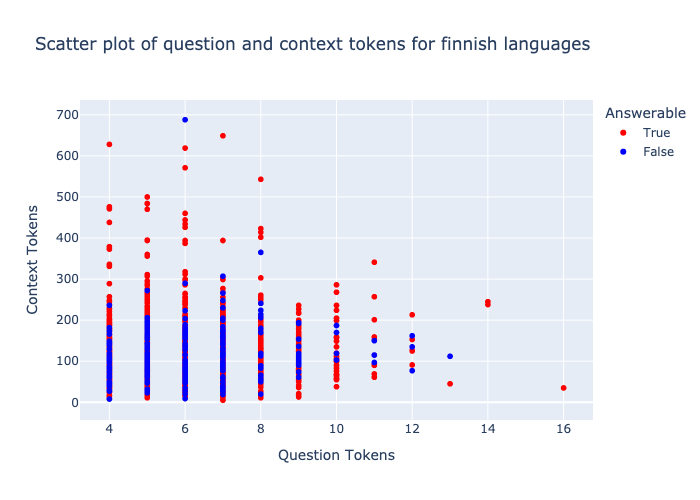
\includegraphics[width=0.25\textwidth]{week1_c_scatter_fi.png}
    \caption{Scatter plot for Finnish}
    \label{fig:scatter_week1_c_fi}
\end{figure}

\begin{figure}[ht]
    \centering
    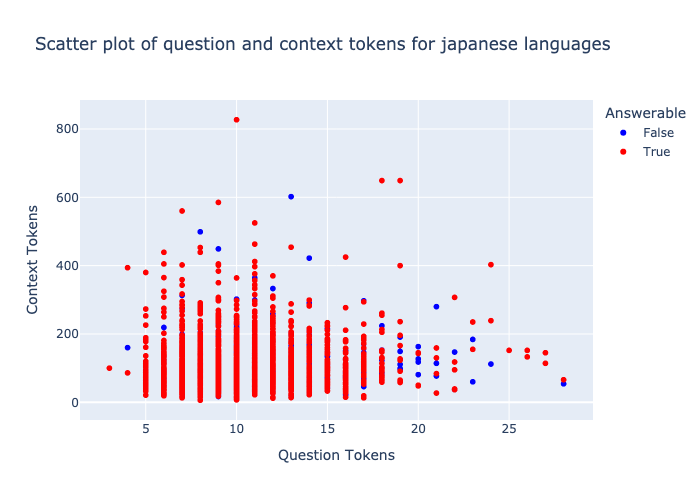
\includegraphics[width=0.25\textwidth]{week1_c_scatter_ja.png}
    \caption{Scatter plot for Japanese}
    \label{fig:scatter_week1_c_ja}
\end{figure}

\begin{figure}[ht]
    \centering
    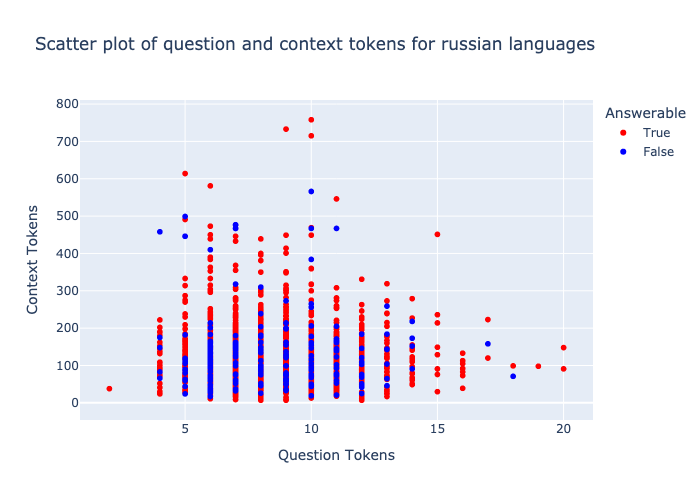
\includegraphics[width=0.25\textwidth]{week1_c_scatter_ru.png}
    \caption{Scatter plot for Russian}
    \label{fig:scatter_week1_c_ru}
\end{figure}

%% distillbert training logs

\begin{table}[ht]
    \centering
    \begin{tabular}{|c|c|c|c|}
        \hline
        Epoch & Language & Exact Match & F1 Score \\
        \hline
        0 & Finnish (fi) & 16.10 & 17.27 \\
        0 & Japanese (ja) & 19.96 & 16.49 \\
        0 & Russian (ru) & 12.88 & 17.24 \\
        \hline
        2 & Finnish (fi) & 21.97 & 22.98 \\
        2 & Japanese (ja) & 26.32 & 17.64 \\
        2 & Russian (ru) & 19.95 & 22.00 \\
        \hline
        4 & Finnish (fi) & 27.27 & 27.39 \\
        4 & Japanese (ja) & 21.27 & 19.28 \\
        4 & Russian (ru) & 18.94 & 21.50 \\
        \hline
        6 & Finnish (fi) & 28.22 & 27.37 \\
        6 & Japanese (ja) & 22.59 & 17.74 \\
        6 & Russian (ru) & 18.94 & 21.27 \\
        \hline
        8 & Finnish (fi) & 27.27 & 26.68 \\
        8 & Japanese (ja) & 23.25 & 18.49 \\
        8 & Russian (ru) & 18.43 & 22.26 \\
        \hline
        10 & Finnish (fi) & 27.08 & 27.51 \\
        10 & Japanese (ja) & 21.93 & 19.07 \\
        10 & Russian (ru) & 16.92 & 21.07 \\
        \hline
    \end{tabular}
    \caption{Evaluation metrics for different languages at various epochs}
    \label{tab:evaluation_metrics}
\end{table}




\subsection{Hyperlinks}

Users of older versions of \LaTeX{} may encounter the following error during compilation:
\begin{quote}
\verb|\pdfendlink| ended up in different nesting level than \verb|\pdfstartlink|.
\end{quote}
This happens when pdf\LaTeX{} is used and a citation splits across a page boundary. The best way to fix this is to upgrade \LaTeX{} to 2018-12-01 or later.

\subsection{Citations}

\begin{table*}
  \centering
  \begin{tabular}{lll}
    \hline
    \textbf{Output}           & \textbf{natbib command} & \textbf{ACL only command} \\
    \hline
    \citep{Gusfield:97}       & \verb|\citep|           &                           \\
    \citealp{Gusfield:97}     & \verb|\citealp|         &                           \\
    \citet{Gusfield:97}       & \verb|\citet|           &                           \\
    \citeyearpar{Gusfield:97} & \verb|\citeyearpar|     &                           \\
    \citeposs{Gusfield:97}    &                         & \verb|\citeposs|          \\
    \hline
  \end{tabular}
  \caption{\label{citation-guide}
    Citation commands supported by the style file.
    The style is based on the natbib package and supports all natbib citation commands.
    It also supports commands defined in previous ACL style files for compatibility.
  }
\end{table*}

Table~\ref{citation-guide} shows the syntax supported by the style files.
We encourage you to use the natbib styles.
You can use the command \verb|\citet| (cite in text) to get ``author (year)'' citations, like this citation to a paper by \citet{Gusfield:97}.
You can use the command \verb|\citep| (cite in parentheses) to get ``(author, year)'' citations \citep{Gusfield:97}.
You can use the command \verb|\citealp| (alternative cite without parentheses) to get ``author, year'' citations, which is useful for using citations within parentheses (e.g. \citealp{Gusfield:97}).

A possessive citation can be made with the command \verb|\citeposs|.
This is not a standard natbib command, so it is generally not compatible
with other style files.

\subsection{References}

\nocite{Ando2005,andrew2007scalable,rasooli-tetrault-2015}

The \LaTeX{} and Bib\TeX{} style files provided roughly follow the American Psychological Association format.
If your own bib file is named \texttt{custom.bib}, then placing the following before any appendices in your \LaTeX{} file will generate the references section for you:
\begin{quote}
\begin{verbatim}
\bibliography{custom}
\end{verbatim}
\end{quote}

You can obtain the complete ACL Anthology as a Bib\TeX{} file from \url{https://aclweb.org/anthology/anthology.bib.gz}.
To include both the Anthology and your own .bib file, use the following instead of the above.
\begin{quote}
\begin{verbatim}
\bibliography{anthology,custom}
\end{verbatim}
\end{quote}

Please see Section~\ref{sec:bibtex} for information on preparing Bib\TeX{} files.

\subsection{Equations}

An example equation is shown below:
\begin{equation}
  \label{eq:example}
  A = \pi r^2
\end{equation}

Labels for equation numbers, sections, subsections, figures and tables
are all defined with the \verb|\label{label}| command and cross references
to them are made with the \verb|\ref{label}| command.

This an example cross-reference to Equation~\ref{eq:example}.


\appendix
\section{Appendix}
\label{app:prompting}
The following Python code demonstrates the prompting setup used for the encoder-decoder model:


\begin{lstlisting}[language=Python]

    def gen_system_message(message: str):
        return f"""
        The following is a qa task, given the context and question, answer the question.The answer will be in the context.
        {message}
        If the question is not answerable, output: "None".
        """
    INLANG_SYSTEM_MESSAGE = gen_system_message('You should answer in the same language as the question.')
    EN_SYSTEM_MESSAGE = gen_system_message('You should answer in English.')
    
    
    def construct_prompt(
        tokenizer : AutoTokenizer,
        question : str,
        context : str,
        answer : Optional[str] = None,
        tokenize : bool = False,
        is_inlang : bool = False
    ) -> str:
        
        messages = [
            {"role": "system", "content": f"{INLANG_SYSTEM_MESSAGE if is_inlang else EN_SYSTEM_MESSAGE}"},
            {"role": "system", "content": f"Context: {context}"},
            {"role": "user", "content": f"Question: {question}"},
        ]
        if answer:
            messages.append({"role": "assistant", "content": f"{answer}"})
    
        prompt = tokenizer.apply_chat_template(
            conversation=messages, 
            tokenize=tokenize, 
            add_generation_prompt=False, 
            format="chatml"
        )
        
        if not answer:
            added = f'<|start_header_id|>assistant<|end_header_id|>'
            prompt = prompt + added
            
        return prompt
\end{lstlisting}





\section{Bib\TeX{} Files}
\label{sec:bibtex}


\end{document}